\subsubsection{Competidores}\label{secsec:competidores}

    No ecossistema de desenvolvimento \textit{low-code}, existem várias plataformas que competem com OutSystems. A escolha entre estas dependerá das necessidades específicas de cada projeto, das preferências da equipa e das metas da empresa. 

    Apesar de OutSystems ser uma das plataformas mais maduras e bem desenvolvidas para este fim no mercado, podemos fazer uma análise dos seus pontos fortes e fracos:

    \textbf{Pontos Fortes:}
    \begin{itemize}
        \item O Controlo de versionamento pode ser integrado com Git e plataformas como GitHub ou GitLab;
        \item Várias opções para integração com outras plataformas com ferramentas como o \href{https://integrationbuilder.outsystems.com/}{Integration Builder}, desde servidores SQL ao MS SharePoint Online;
        \item Vastas livrarias, pré-definições, e templates disponíveis;
        \item Ênfase também no desenvolvimento de aplicações móveis.
    \end{itemize}

    \textbf{Pontos Fracos:}
    \begin{itemize}
        \item Uma personalização de UI menos flexível em comparação com algumas alternativas;
        \item Flexibilidade para correr os próprios servidores está apenas disponível em alguns planos;
        \item Colaboração não é um dos aspetos mais fortes da plataforma;
        \item Custo comparativamente elevados em relação a outras alternativas\cite{outsystems-vs-mendix}.
    \end{itemize}

    Na Figura \ref{fig:googletrendslowcodeplatforms-ui} pode-se ver algumas das plataformas \textit{low-code} mais usadas nos últimos cinco anos de acordo com o Google Trends e na Figura \ref{tab:lowcode-comparison} como se comparam com as demais.

    \begin{figure}[p] % htbp
        \centering
        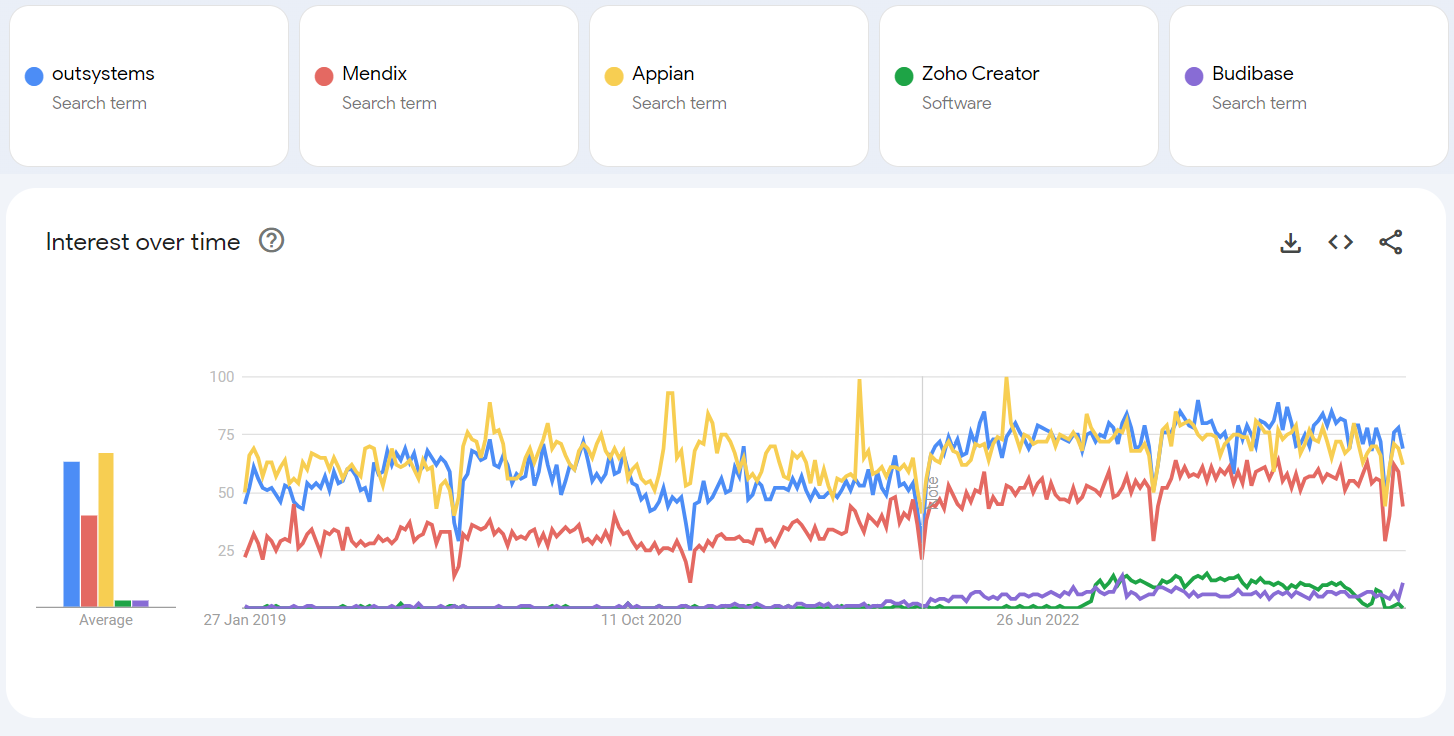
\includegraphics[width=\textwidth]{imgs/GoogleTrendsLowCodePlatforms.png}
        \caption{Google Trends for Low Code Platforms Worldwide}\label{fig:googletrendslowcodeplatforms-ui}
        \source{\cite{g-trends-low-code-platforms}}
    \end{figure}

    % Use this to finish the table: https://impalaintech.com/blog/mendix-vs-outsystems-vs-appian/

    \begin{table}[p] % htbp
        \centering
        \caption{Comparação de Plataformas Low-Code}
        \label{tab:lowcode-comparison}
        \source{\cite{mendix-vs-outsystems-vs-appian,outsystems-vs-mendix}} 
        \begin{tblr}{
            % example for tblr: https://tex.stackexchange.com/questions/603349/tabularray-and-new-command-for-multicolumn-cells
            % another example: https://tex.stackexchange.com/questions/605676/tabularray-how-to-control-the-vertical-alignment-of-the-cells-contents
            hlines={lightgray}, vlines={lightgray},
            width = \linewidth,% total width set to width available
            %rows = {c,m}, % c aligns horizontally, m aligns vertically, aligns all rows
            colspec={Q[l,m,3cm] X[c,m] X[c,m] X[c,m] X[c,m]},
            cell{1}{1} = {r=2}{c}, % Merge cells in the first row and second row
        }
            \textbf{Campo} & \SetCell[c=4]{c} \textbf{Plataformas} \\
                        & \textbf{OutSystems} & \textbf{Mendix} & \textbf{Appian} & \textbf{Pega} \\ 
            Facilidade de Utilização               & Médio       & Alto        & Alto        & Baixo        \\ 
            Integração                             & Muito Alto  & Alto        & Alto        & Alto        \\ 
            Escalabilidade                         & Muito Alto  & Muito Alto  & Muito Alto  & Muito Alto  \\ 
            % Flexibilidade no Desenvolvimento da UI & Alto        & Muito Alto  & Alto        & Alto        \\  % Para Pega e Appian são as unicas duas que não estão bem fundamentadas
            Foco em Desenvolvimento Móvel          & Alto        & Alto        & Alto        & Alto        \\ 
            Colaboração                            & Alto        & Muito Alto  & Alto        & Alto       \\
            Custo                                  & Alto        & Disponível após Pedido & Alto & Disponível após Pedido  \\
        \end{tblr}
        % 1- https://impalaintech.com/blog/mendix-vs-outsystems-vs-appian/
    \end{table}

    O ambiente de desenvolvimento \textit{low-code} é muito competitivo, pelo que existe uma panóplia de ferramentas com objetivos similares, como por exemplo: Bonitasoft, Appsheet, Bubble, Zoho Create, Budibase, Backendless, Eclipse/SAP, Salesforce Lightning, etc. Pode ser que nenhuma ferramenta ou combinação entre as ferramentas aqui analisadas seja a mais indicada para qualquer projeto. Algumas equipas também adotam abordagens com uma pilha de infraestrutura constituída por vários programas de ecossistemas diferentes, utilizando diferentes ferramentas para aspetos específicos, como Webflow para o front-end e Zappier ou N8n para o lado do servidor. No fundo, esta área é muito flexível e está sempre em constante evolução, e pode ser que a infraestrutura mais indicada para um projeto seja uma que tenha que ser feita à medida.
        
    % Reddit opinion: https://www.reddit.com/r/lowcode/comments/lp9f4p/recommendations_please/
    % Outras: Bonitasoft, Appsheet, bubble, Zoho Create, Budibase, Backendless and Eclipse/SAP, Salesforce Lightning
    % ou uso de várias: Webflow is relatively powerful for a front-end, Zappier or N8n (free) - for the server side, and some database (tool) - Airtable/Firebase/Backendless - for the data.
    % outra dessas arranjei aqui: https://www.outsystems.com/forums/discussion/86088/outsystems-vs-other-low-code-platforms/

    % Another reddit opinion: https://www.reddit.com/r/lowcode/comments/lp9f4p/recommendations_please/

    \subsubsubsection{Mendix}\label{secsecsec:mendix}
        
        Fundada em 2005, a Mendix é uma plataforma de desenvolvimento \textit{low-code} projetada para fornecer às empresas ferramentas para rapidamente construir e distribuir aplicações personalizadas. Os fundadores acreditavam que o desenvolvimento e a distribuição de software iria beneficiar bastante com uma mudança de paradigma, e daí nasceu a empresa. Mendix foca-se na colaboração permitindo às equipas trabalhar efetivamente em conjunto e simplificando o desenvolvimento através de modelagem visual com uma interface intuitiva, como visível na Figura \ref{fig:mendixui-ui}, e componentes reutilizáveis\cite{why-was-mendix-founded}.

        O Mendix destaca-se pela sua flexibilidade enquanto mantém um bom nível de intuição. Oferece também um mercado privado de aplicações que permite a sua partilha mesmo internamente. Proporciona uma variedade de opções de implementação, incluindo diferentes serviços cloud, soluções locais e híbridas, adaptando-se sempre às diversas necessidades da organização\cite{outsystems-vs-mendix}.

        \begin{figure}[htbp] % htbp
            \centering
            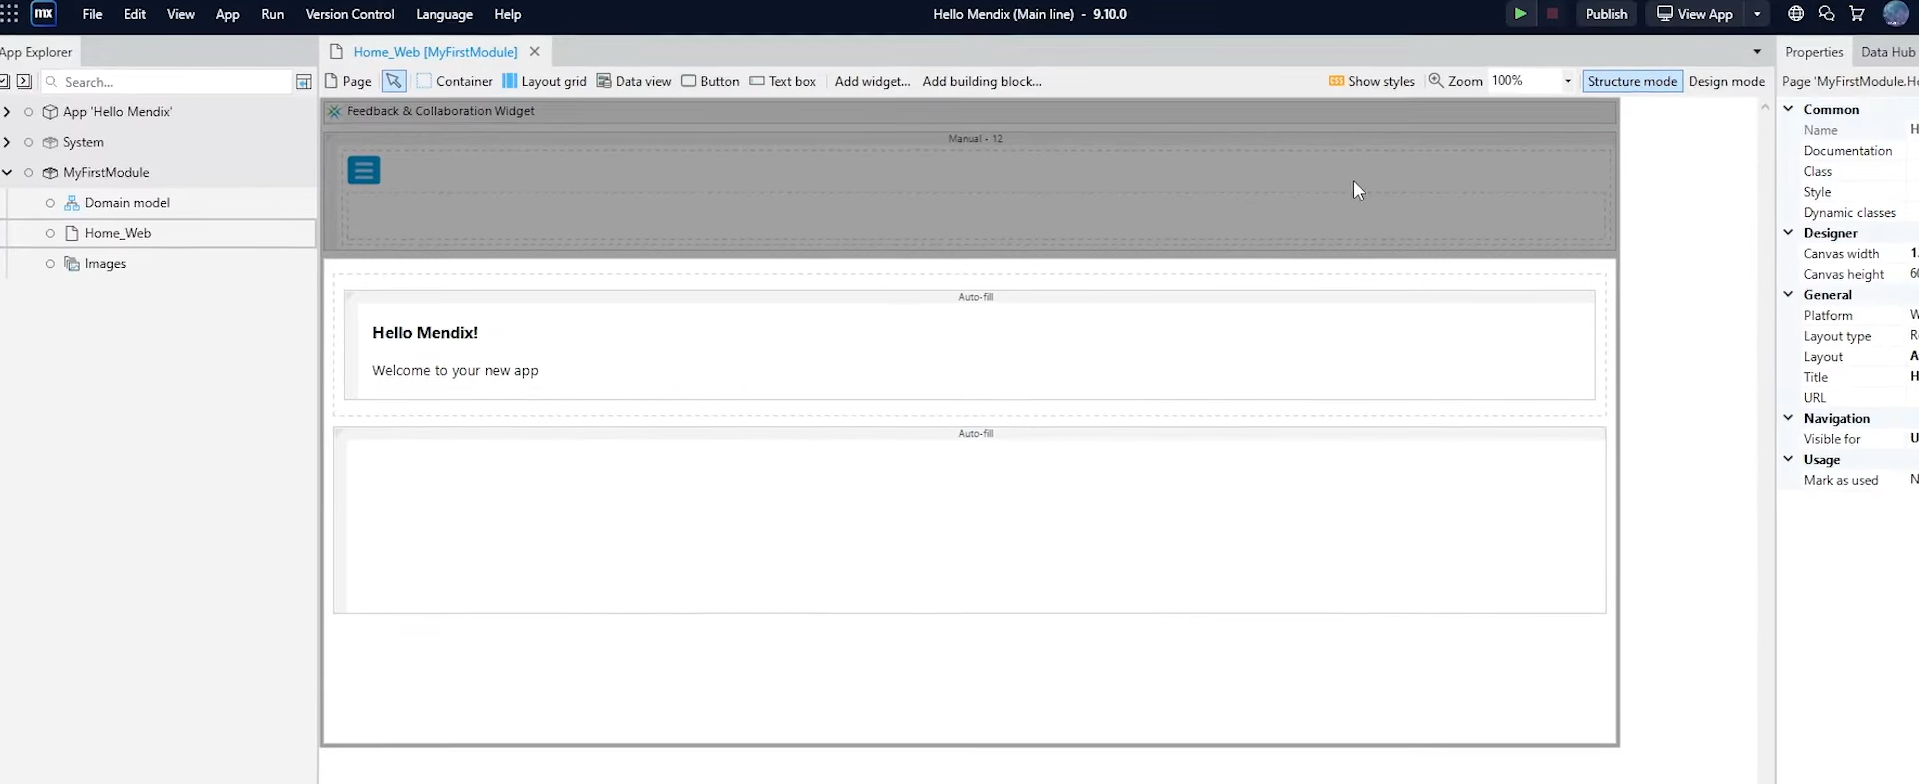
\includegraphics[width=\textwidth]{imgs/MendixUI.png}
            \caption{Mendix UI}\label{fig:mendixui-ui}
            \source{\cite{mendix-ui}}
        \end{figure}

        % https://www.appsmith.com/blog/mendix-vs-outsystems

    \subsubsubsection{Appian}\label{secsec:appian}

        Fundada em 1999 por Michael Beckley, Robert Kramer, Marc Wilson e Matthew Calkins e com uma interface como observável na Figura \ref{fig:appian-ui}, a Appian é uma plataforma de desenvolvimento \textit{low-code} criada com o objetivo de simplificar e acelerar o processo de desenvolvimento de software e com a visão de que pessoas talentosas e com paixão, quando proporcionadas com as ferramentas certas irão dar resultados incríveis\cite{appian-company-history,appian-company-overview}. 
    
        \begin{figure}[htbp] % htbp
            \centering
            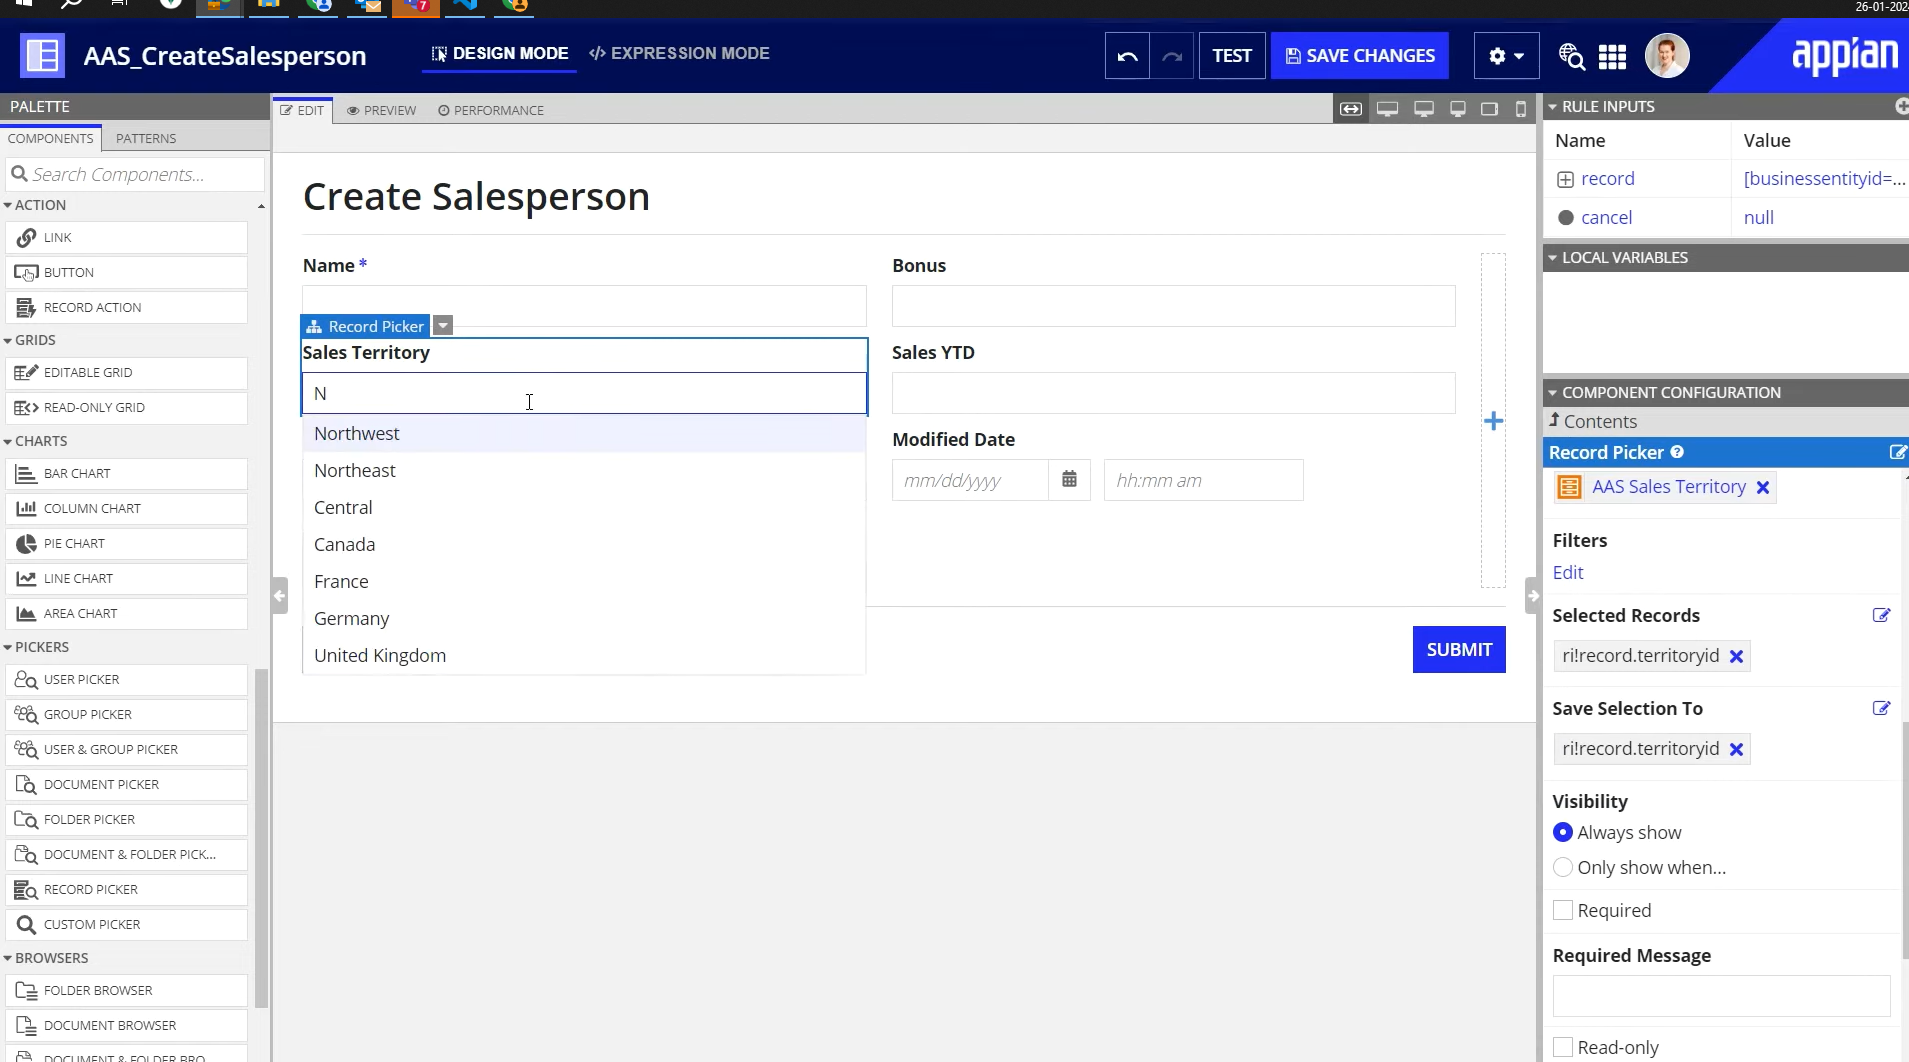
\includegraphics[width=\textwidth]{imgs/AppianUI.png}
            \caption{Appian UI}\label{fig:appian-ui}
            \source{\cite{mendix-ui}}
        \end{figure}

        Appian destaca-se no mercado de desenvolvimento de software devido a várias funcionalidades distintas. Algumas delas incluem:
        
        \begin{enumerate}
            \item \textbf{\textit{Deployment} Eficiente:}
                \begin{itemize}
                    \item Permite a implantação rápida de aplicações com variadas ferramentas de implantação;
                    \item Oferece a sua própria solução para controlo de versionamento.
                \end{itemize}
            
            \item \textbf{Vários Formatos para Apresentação de Dados:}
                \begin{itemize}
                    \item Possibilita apresentar dados em vários formatos, como tabelas, gráficos em formato grade e PDF.
                \end{itemize}
            
            \item \textbf{Desenvolvimento Visual:}
                \begin{itemize}
                    \item Programadores podem moldar fluxogramas para criar diagramas de processos de forma visual, eliminando a necessidade de codificar manualmente.
                \end{itemize}
            
            \item \textbf{Pontos a Considerar (Desvantagens):}
                \begin{itemize}
                    \item Processo de documentação precisa de ser aprimorado;
                    \item Limitações na integração com outros produtos;
                    \item A ferramenta de gestão de permissões pode ser um pouco lenta;
                    \item Desenvolvimento geral de aplicações pode ser mais lento em comparação com as alternativas analisadas.
                \end{itemize}
        \end{enumerate}
        
        Appian destaca-se na eficiência da implantação de aplicações e na criação de processos através de fluxogramas visuais. A sua flexibilidade na apresentação de dados, em junção com a capacidade de desenvolver aplicações para diversos setores, fazem dela uma opção bastante versátil\cite{mendix-vs-outsystems-vs-appian}.

    \subsubsubsection{Pega Platform}\label{secsecsec:pega}
    
        % fundada https://www.pega.com/about/leadership/alan-trefler#:~:text=Inspired%2C%20he%20founded%20Pega%20in,today%20known%20as%20low%2Dcode.

        A Pega Platform, a plataforma mais antiga das analisadas, fundada em 1983, foi criada por Alan Trefler, um programador na área financeira e dos seguros, fundou Pega devido à desconexão que existia entre os métodos tecnológicos usados e os processos e objetivos empresariais. Desde então, a plataforma tem desempenhado um papel crucial no cenário de desenvolvimento de software, fornecendo soluções robustas para diversas necessidades empresariais, a sua interface está representada na Figura \ref{fig:pega-ui}.

        \begin{figure}[htbp] % htbp
            \centering
            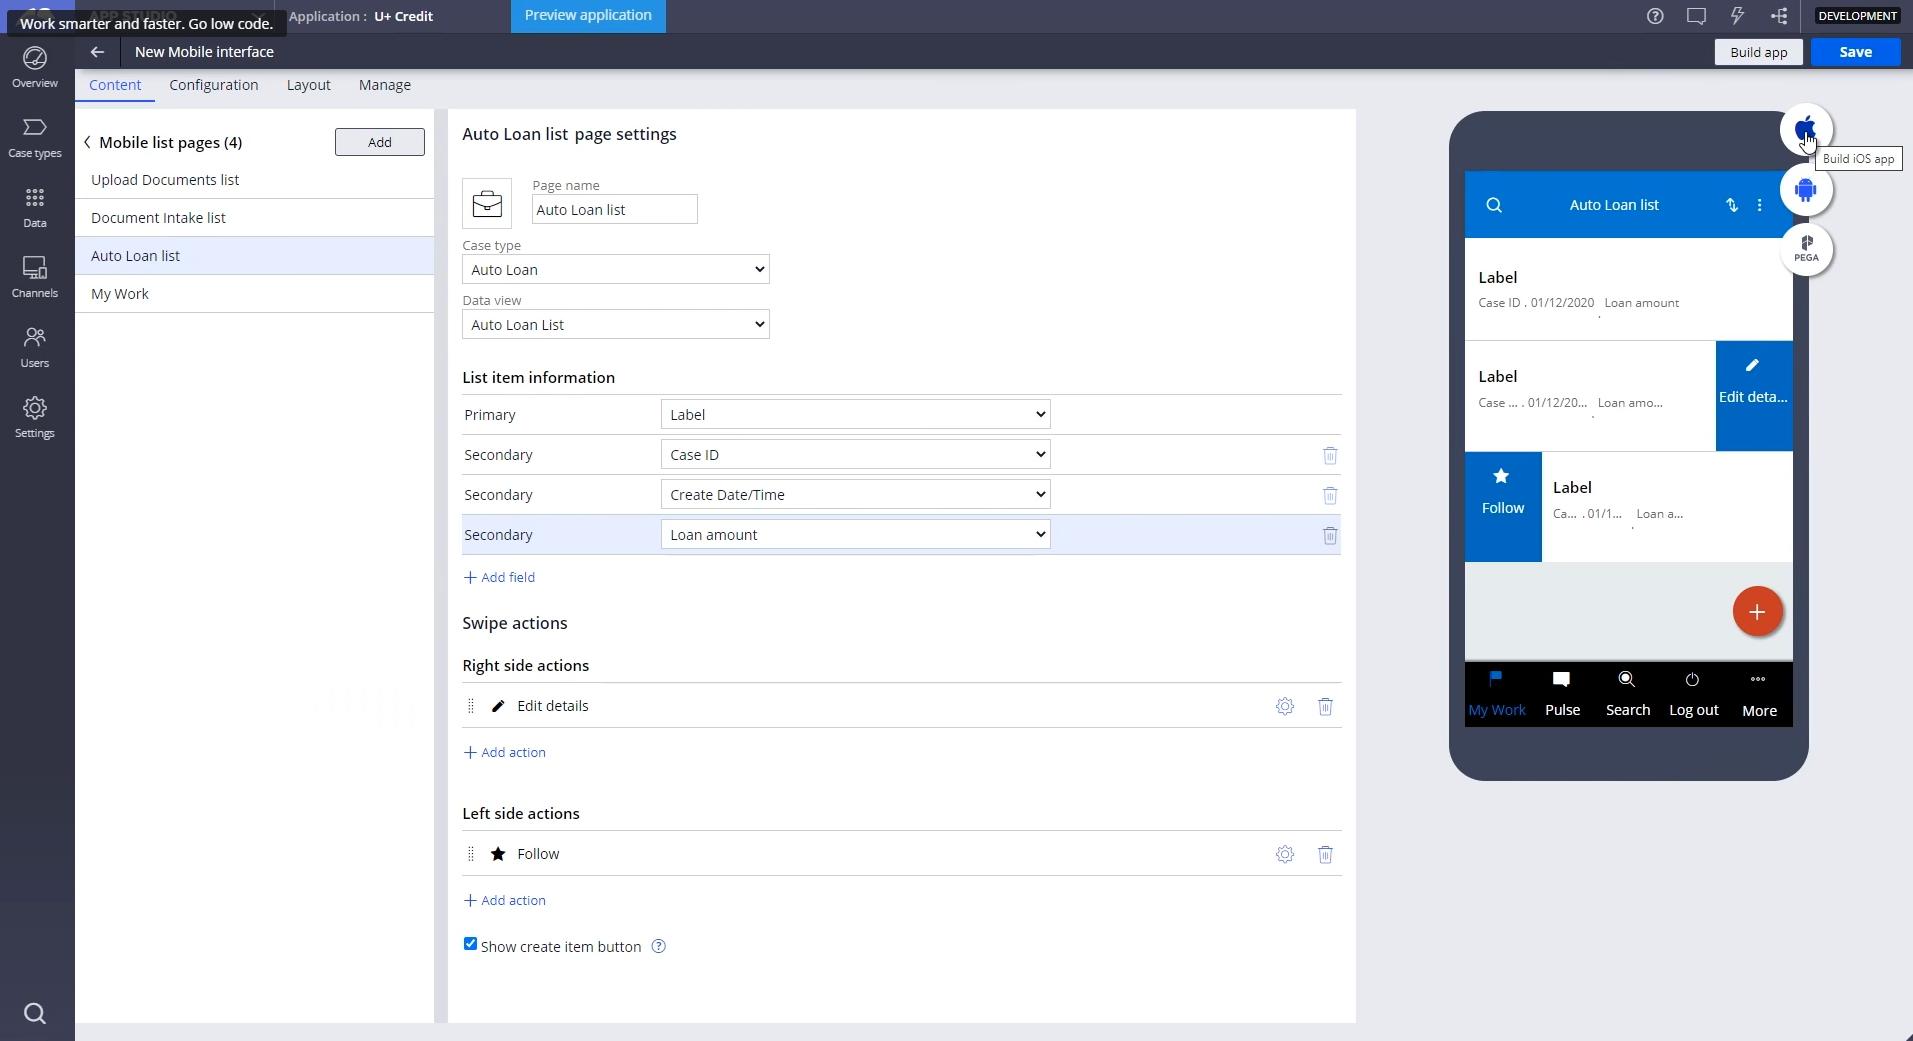
\includegraphics[width=\textwidth]{imgs/PegaUI.png} % You can replace 'example-image-a' with the path to your actual image
            \caption{Pega UI}\label{fig:pega-ui}
            \source{\cite{pega-ui}}
        \end{figure}

        Algumas vantagens e desvantagens da plataforma incluem:
    
        \begin{itemize}
        \item \textbf{Vantagens:}
            \begin{itemize}
            \item Oferece uma abordagem eficiente na gestão de casos, utilizando um modelo central que permite controlar tarefas, contribuindo para uma integração forte com os paradigmas das empresas\cite{o-que-e-gestao-de-casos-pega};
            \item Forte capacidade de incorporar e utilizar inteligência artificial nas aplicações.
            \end{itemize}
        
        \item \textbf{Desvantagens:}
            \begin{itemize}
            \item Tem uma curva de aprendizagem mais acentuada.
            \end{itemize}
        \end{itemize}    